
\begin{figure}[H]
  {
    \setlength{\tabcolsep}{3.0pt}
    \setlength\cmidrulewidth{\heavyrulewidth} % Make cmidrule = 
    \begin{adjustbox}{width=3cm,center}
      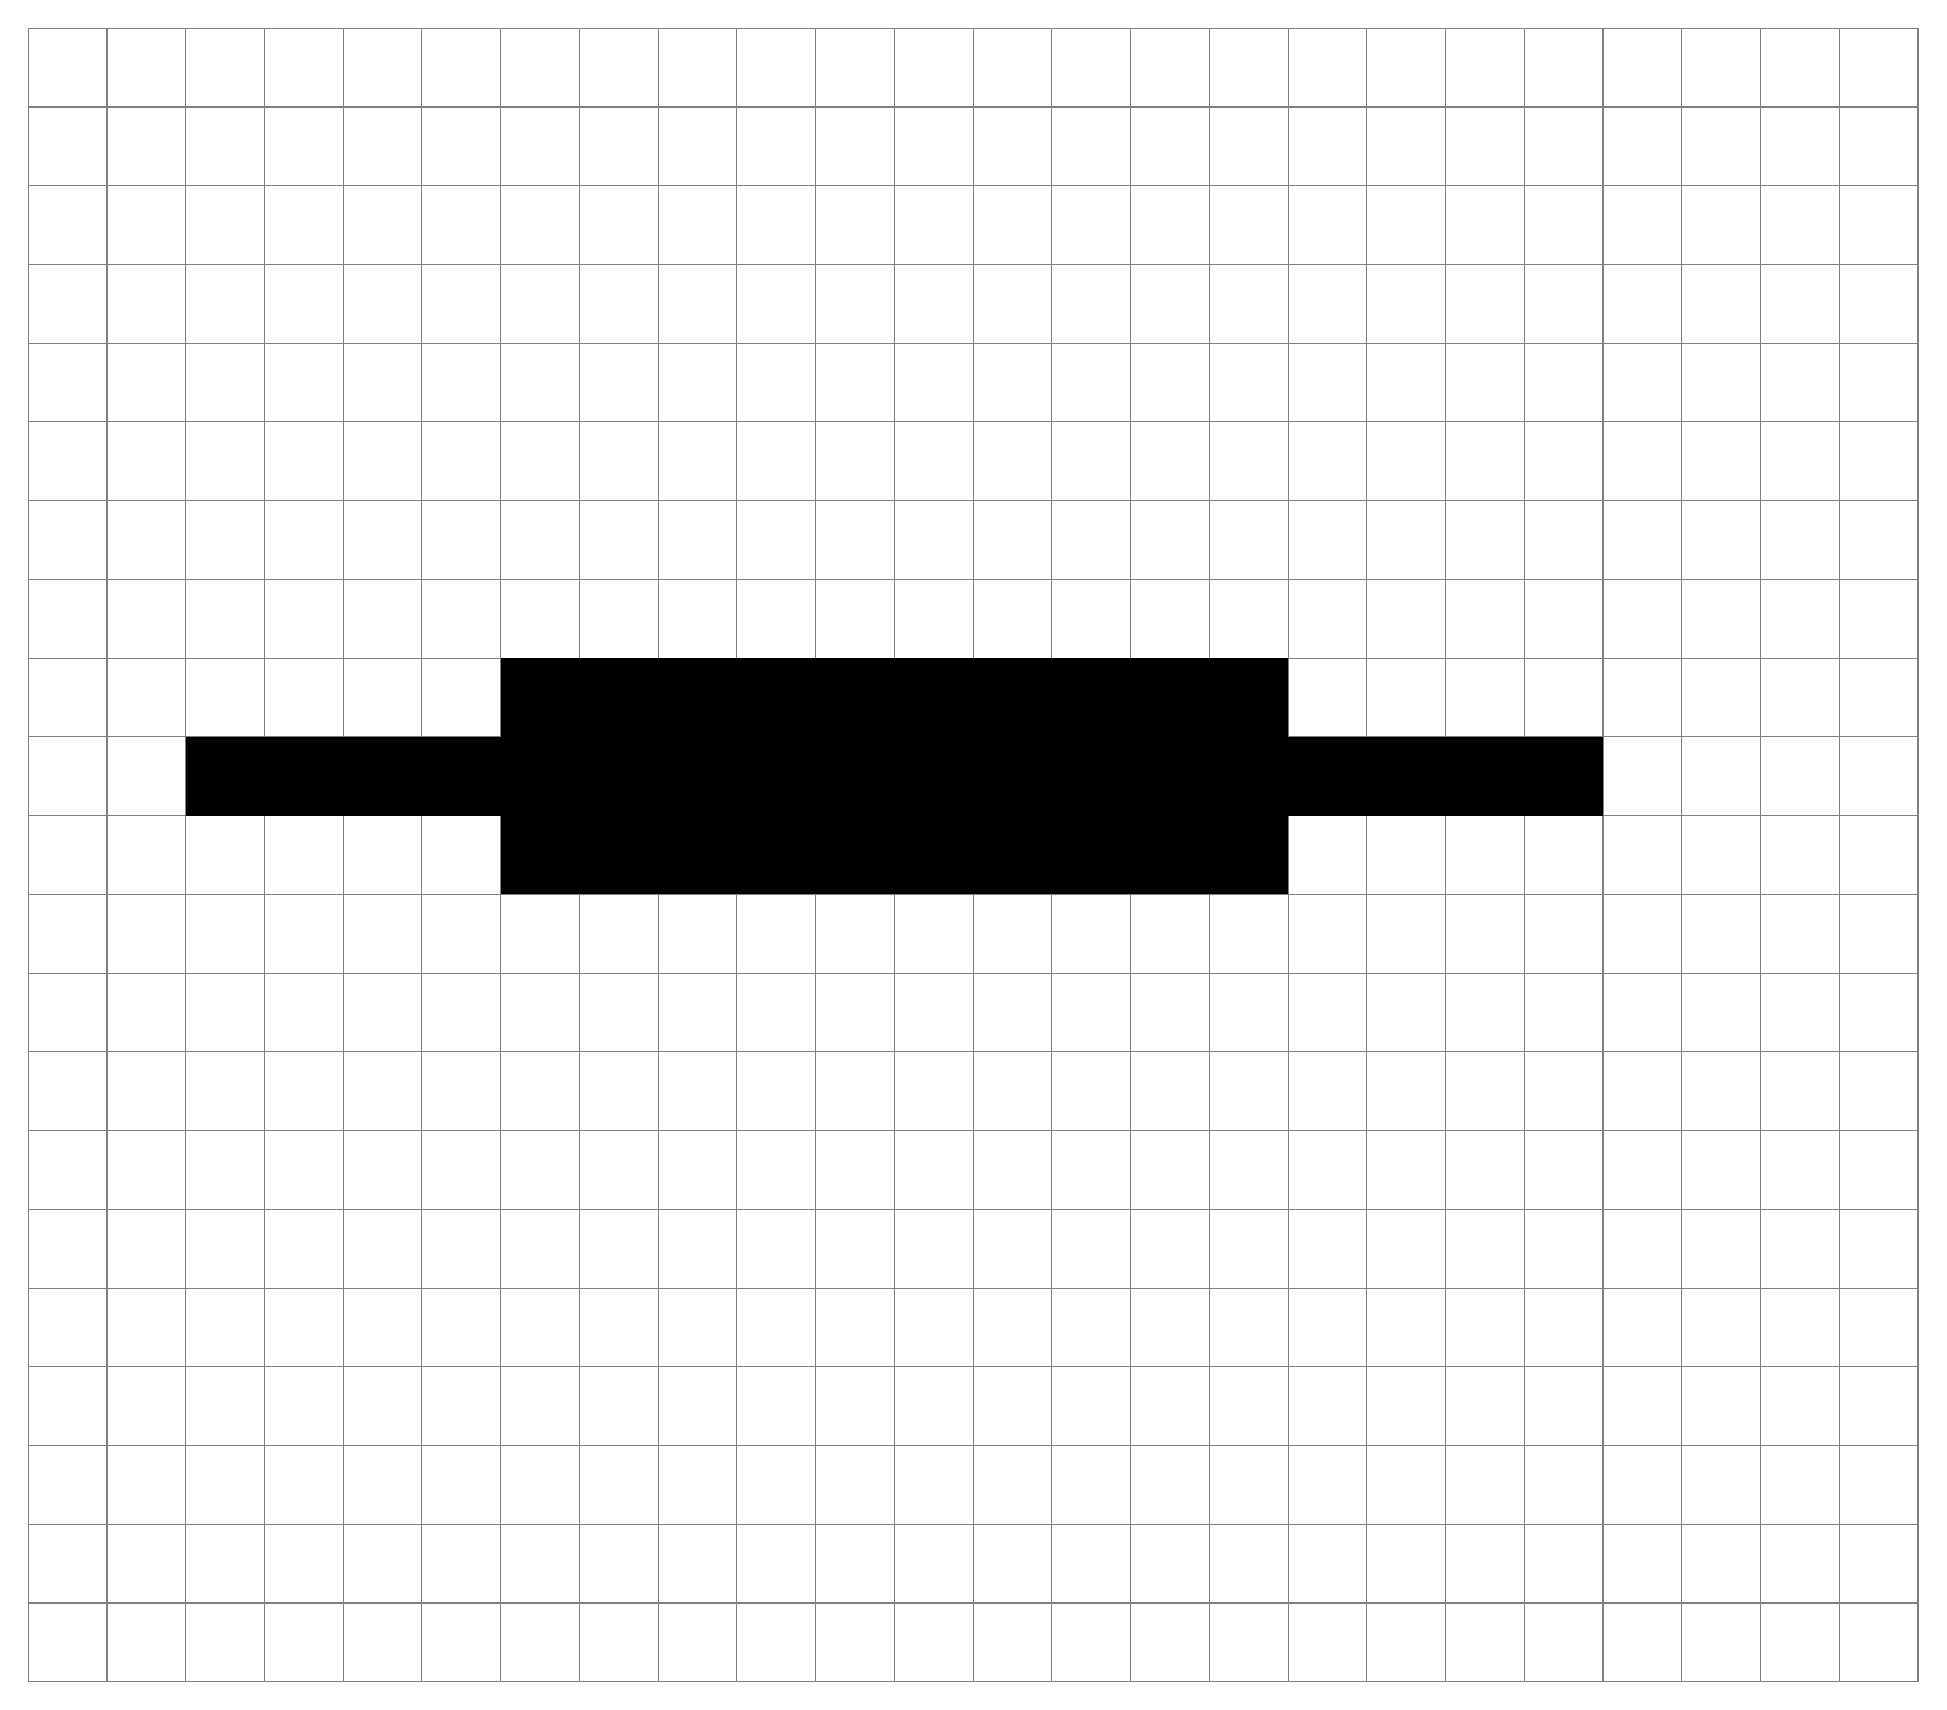
\begin{tikzpicture}

	\draw[step=1.0,gray,thin] (0,0) grid (24,21);
	\fill[\MULTICOLORTWO] (6,12) rectangle ++ (1,1);
	\fill[\MULTICOLORTWO] (7,12) rectangle ++ (1,1);
	\fill[\MULTICOLORTWO] (8,12) rectangle ++ (1,1);
	\fill[\MULTICOLORTWO] (9,12) rectangle ++ (1,1);
	\fill[\MULTICOLORTWO] (10,12) rectangle ++ (1,1);
	\fill[\MULTICOLORTWO] (11,12) rectangle ++ (1,1);
	\fill[\MULTICOLORTWO] (12,12) rectangle ++ (1,1);
	\fill[\MULTICOLORTWO] (13,12) rectangle ++ (1,1);
	\fill[\MULTICOLORTWO] (14,12) rectangle ++ (1,1);
	\fill[\MULTICOLORTWO] (15,12) rectangle ++ (1,1);
	\fill[\MULTICOLORTWO] (2,11) rectangle ++ (1,1);
	\fill[\MULTICOLORTWO] (3,11) rectangle ++ (1,1);
	\fill[\MULTICOLORTWO] (4,11) rectangle ++ (1,1);
	\fill[\MULTICOLORTWO] (5,11) rectangle ++ (1,1);
	\fill[\SPRITECOLOR] (6,11) rectangle ++ (1,1);
	\fill[\SPRITECOLOR] (7,11) rectangle ++ (1,1);
	\fill[\SPRITECOLOR] (8,11) rectangle ++ (1,1);
	\fill[\SPRITECOLOR] (9,11) rectangle ++ (1,1);
	\fill[\SPRITECOLOR] (10,11) rectangle ++ (1,1);
	\fill[\SPRITECOLOR] (11,11) rectangle ++ (1,1);
	\fill[\SPRITECOLOR] (12,11) rectangle ++ (1,1);
	\fill[\SPRITECOLOR] (13,11) rectangle ++ (1,1);
	\fill[\SPRITECOLOR] (14,11) rectangle ++ (1,1);
	\fill[\SPRITECOLOR] (15,11) rectangle ++ (1,1);
	\fill[\MULTICOLORTWO] (16,11) rectangle ++ (1,1);
	\fill[\MULTICOLORTWO] (17,11) rectangle ++ (1,1);
	\fill[\MULTICOLORTWO] (18,11) rectangle ++ (1,1);
	\fill[\MULTICOLORTWO] (19,11) rectangle ++ (1,1);
	\fill[\MULTICOLORTWO] (6,10) rectangle ++ (1,1);
	\fill[\MULTICOLORTWO] (7,10) rectangle ++ (1,1);
	\fill[\MULTICOLORTWO] (8,10) rectangle ++ (1,1);
	\fill[\MULTICOLORTWO] (9,10) rectangle ++ (1,1);
	\fill[\MULTICOLORTWO] (10,10) rectangle ++ (1,1);
	\fill[\MULTICOLORTWO] (11,10) rectangle ++ (1,1);
	\fill[\MULTICOLORTWO] (12,10) rectangle ++ (1,1);
	\fill[\MULTICOLORTWO] (13,10) rectangle ++ (1,1);
	\fill[\MULTICOLORTWO] (14,10) rectangle ++ (1,1);
	\fill[\MULTICOLORTWO] (15,10) rectangle ++ (1,1);

      \end{tikzpicture}
    \end{adjustbox}
  }\caption{TEARDROP\_EXPLOSION3}
\end{figure}
